
\chapter{KESIMPULAN DAN SARAN}

\section{Kesimpulan}
Berdasarkan hasil dan pembahasan terkait empat Model \textit{CNN} dalam tugas Prediksi Pose Semaphore Berbasis Deep Learning dapat diperoleh beberapa kesimpulan tentang kinerja masing-masing model. Selain kinerja masing-masing model juga dibahas tentang pengujian dilakukan dengan membandingkan performa Model \textit{CNN}, Model \textit{CNN2}, \textit{ResNet50V2}, dan \textit{Xception} dalam mengenali pose semaphore yang dihasilkan oleh sembilan koresponden berbeda dengan lima variasi gerakan dari huruf A hingga E. Berikut ini kesimpulan yang bisa diperoleh 
\begin{enumerate}[nolistsep]

\item Perbandingan hasil \textit{loss} dari keempat model (Model CNN, Model \textit{CNN2}, \textit{ResNet50V2}, dan \textit{Xception}) pada Gambar \ref{fig:GrafikPerbandinganLoss} memberikan gambaran kuantitatif tentang performa dan konvergensi masing-masing model selama proses pelatihan. Semakin rendah nilai loss, semakin baik model tersebut dalam menemukan representasi yang tepat dari data dan mengoptimalkan parameter dalam rangka tugas pengenalan pose semaphore 
\begin{figure}[!hbt]
	\centering
	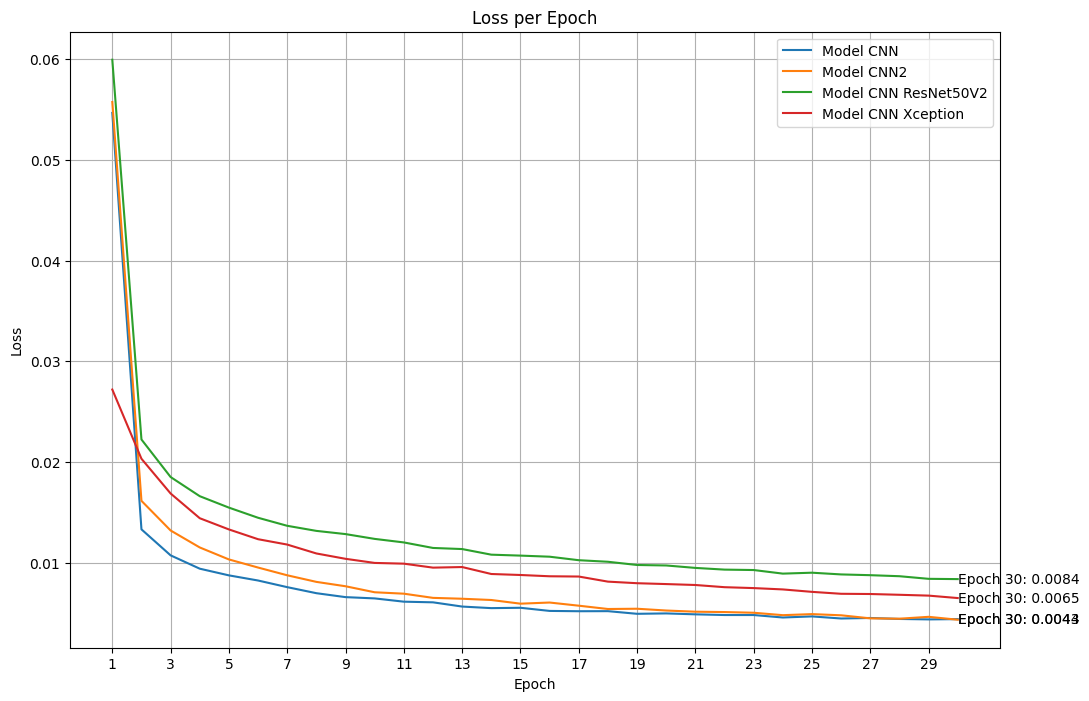
\includegraphics[width=0.7\linewidth]{gambar/bener/Perbandingan_LossCNN.png}
	\captionof{figure}{Grafik Perbandingan Loss}
	\label{fig:GrafikPerbandinganLoss}
\end{figure}
Model \textit{CNN} dan Model \textit{CNN2} menunjukkan hasil yang lebih baik dibandingkan dengan ResNet50V2 dan \textit{Xception}. Dari hasil \textit{loss} yang terekam selama 30 \textit{epoch}, Model \textit{CNN} dan Model \textit{CNN2} mencapai nilai \textit{loss} terendah lebih cepat dan secara konsisten memiliki nilai \textit{loss} yang lebih rendah dibandingkan dua model lainnya.

Model \textit{CNN} mencapai nilai \textit{loss} terendah sekitar 0.0044 pada \textit{epoch} ke-30, sedangkan Model \textit{CNN2} mencapai nilai \textit{loss} terendah sekitar 0.0043 pada \textit{epoch} ke-29. Dalam kasus ini, Model \textit{CNN} dan Model \textit{CNN2} memiliki hasil \textit{loss} yang sangat mendekati satu sama lain, menandakan kualitas representasi yang serupa dalam tugas pengenalan pose semaphore.

Sementara itu, \textit{ResNet50V2} dan \textit{Xception} juga menunjukkan penurunan nilai \textit{loss} yang konsisten selama proses pelatihan. Namun, keduanya memiliki nilai \textit{loss} yang agak lebih tinggi dibandingkan dua model sebelumnya. ResNet50V2 mencapai nilai \textit{loss} terendah sekitar 0.0083 pada \textit{epoch} ke-30, sementara \textit{Xception} mencapai nilai \textit{loss} terendah sekitar 0.0065 pada \textit{epoch} ke-26.

\item Berdasarkan hasil perbandingan akurasi dari empat model sesuai dengan Gambar \ref{fig:GrafikPerbandinganAkurasi}, yaitu Model \textit{CNN}, Model \textit{CNN2}, \textit{ResNet50V2}, dan \textit{Xception}, pada \textit{epoch} terakhir yaitu epich ke-30 . terlihat bahwa Model \textit{CNN2} memiliki akurasi tertinggi pada epoch terakhir, yaitu sekitar 93.53\%. Model ini juga memiliki validasi akurasi yang cukup tinggi, mencapai sekitar 97.20\%. Model \textit{CNN} mengalami performa yang hampir setara dengan Model \textit{CNN2}, dengan akurasi pada epoch terakhir sekitar 93.72\%, dan validasi akurasi sekitar 97.50\%.
\begin{figure}[!hbt]
	\centering
	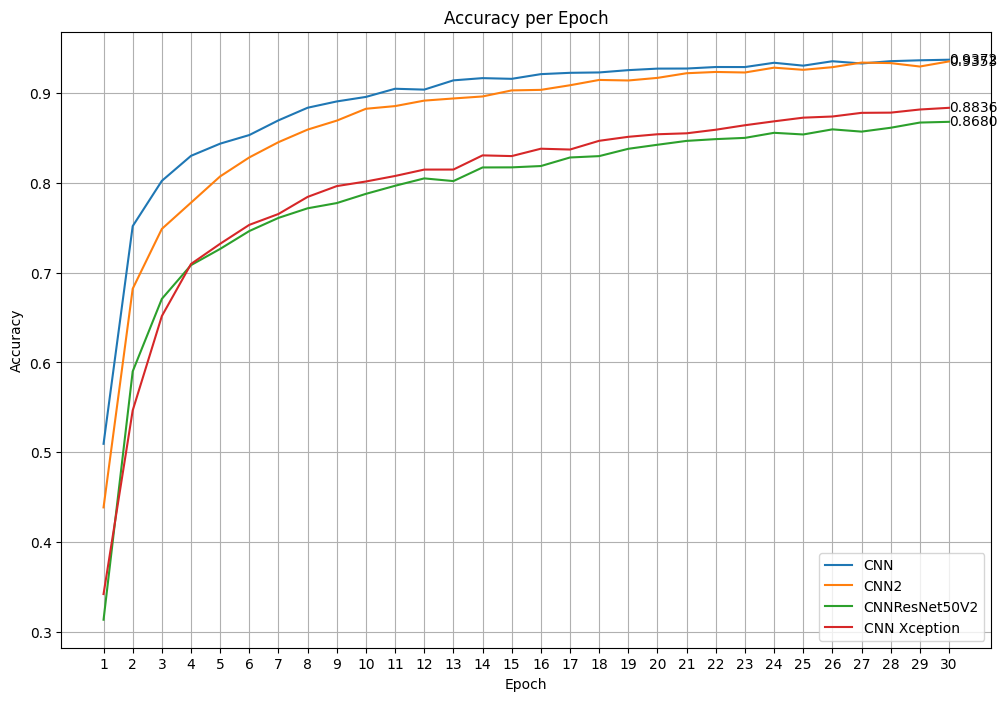
\includegraphics[width=0.7\linewidth]{gambar/bener/Perbandingan_AkurasiCNN.png}
	\captionof{figure}{Grafik Perbandingan Loss}
	\label{fig:GrafikPerbandinganAkurasi}
\end{figure}
Sementara itu, Model \textit{ResNet50V2} dan Model \textit{Xception} memiliki akurasi yang sedikit lebih rendah daripada kedua model \textit{CNN} tersebut. Model \textit{ResNet50V2} mencapai akurasi sekitar 88.36\%, dengan validasi akurasi sekitar 96.59\%. Sedangkan, Model \textit{Xception} memiliki akurasi dan validasi akurasi yang sama dengan Model \textit{ResNet50V2}, yaitu sekitar 88.36\% dan 92.39\% pada epoch terakhir.

Dari hasil ini, dapat disimpulkan bahwa Model \textit{CNN2} adalah yang memiliki akurasi tertinggi pada epoch terakhir, diikuti oleh Model CNN. Meskipun Model \textit{ResNet50V2} dan Model \textit{Xception} memiliki akurasi yang lebih rendah, namun keduanya masih menunjukkan kinerja yang cukup baik dalam tugas klasifikasi pose semaphore.

\item Berdasarkan Hasil Evaluasi Metrik seperti pada Gambar \ref{fig:GrafikPerbandinganEvaluasiMetrik} dari \textit{Precision} , \textit{Recall} dan \textit{F1-Score} dari masing-masing model dapat diambil hasil yaitu Model \textit{CNN} menunjukkan tingkat \textit{precision} sebesar 0.973, \textit{recall} sebesar 0.809, dan \textit{F1-Score} sebesar 0.881. Sementara itu, model \textit{CNN2} mencapai \textit{precision} sebesar 0.968, \textit{recall} sebesar 0.946, dan \textit{F1-Score} sebesar 0.952, menunjukkan performa yang sangat baik dalam mengenali dan memprediksi kelas data.
\begin{figure}[!hbt]
	\centering
	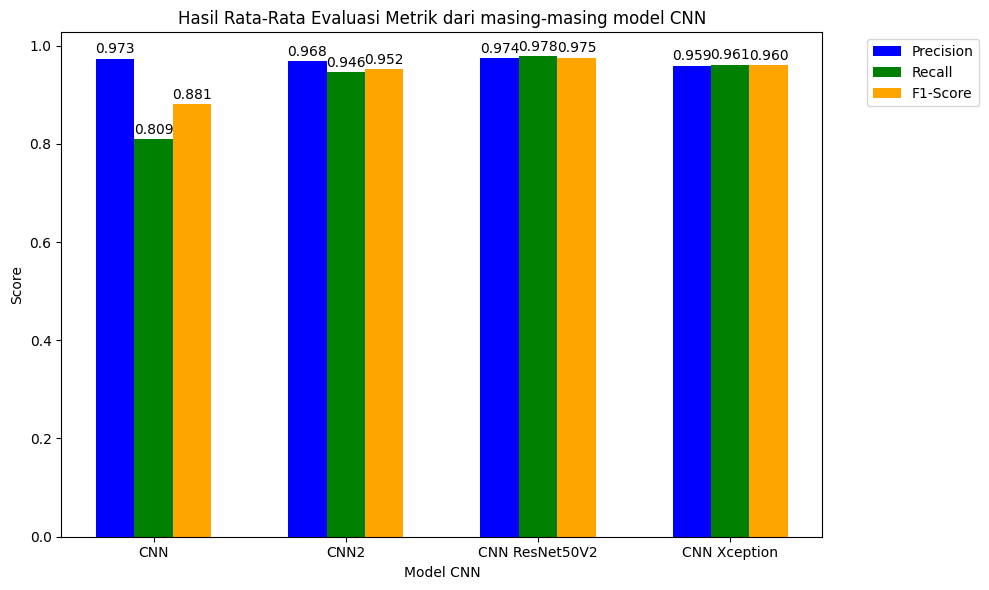
\includegraphics[width=0.7\linewidth]{gambar/bener/RataRataEvaluasiMetrik.png}
	\captionof{figure}{Hasil Rata-Rata Evaluasi Metrik dari masing-masing model CNN}
	\label{fig:GrafikPerbandinganEvaluasiMetrik}
\end{figure}
Selanjutnya, model \textit{CNN} \textit{ResNet50V2} menunjukkan hasil evaluasi yang sangat mengesankan, dengan \textit{precision} mencapai 0.974, \textit{recall} sebesar 0.978, dan \textit{F1-Score} sebesar 0.975. Hal ini menandakan bahwa model \textit{CNN} ResNet50V2 memiliki kemampuan yang sangat tinggi dalam mengenali dan mengklasifikasikan data dengan akurasi tinggi. Terakhir, model \textit{CNN} \textit{Xception} juga menunjukkan performa yang baik, dengan \textit{precision} sebesar 0.959, \textit{recall} sebesar 0.961, dan \textit{F1-Score} sebesar 0.960.

\item Berdasarkan data dari Tabel \ref{tbl:training_time}, dapat disimpulkan bahwa terdapat perbedaan signifikan dalam waktu yang diperlukan dalam pelatihan masing-masing model \textit{CNN} selama 30 \textit{epoch}. Model \textit{CNN2} menunjukkan kinerja yang sangat baik dengan waktu rata-rata pelatihan hanya sekitar 20.02 detik per \textit{epoch}, menjadikannya model yang paling efisien dalam hal waktu. Di sisi lain, model \textit{Xception} dan \textit{ResNet50V2} memerlukan waktu yang lebih lama ketika melakukan pelatihan, dengan rata-rata masing-masing sekitar 194.07 detik dan 192.12 detik per \textit{epoch}
\item Hasil Confusion Matrix dari empat model baik \textit{CNN},\textit{CNN2}, \textit{CNN ResNet50V2}, dan \textit{CNN Xception} telah menghasilkan kuantitatif metrik evaluasi klasifikasi yang memberikan gambaran yang sangat positif terhadap performa setiap model dalam mengenali huruf A sampai E. Masing-masing model mencatatkan \textit{True Positives} (\textit{TP}) yang tinggi bagi setiap huruf, yaitu 41 \textit{TP} dari huruf A, 32 \textit{TP} dari huruf B, 31 \textit{TP} dari huruf C, 33 \textit{TP} dari huruf D, dan 37 \textit{TP} dari huruf E. Hal ini menandakan bahwa keempat model memiliki akurasi yang tinggi dalam mengklasifikasikan huruf-huruf tersebut dengan benar.
\end{enumerate}

\section{Saran}
Sebagai saran pengembangan lebih lanjut dalam penelitian ini, disarankan agar mengadopsi metodologi lain yang dapat meningkatkan analisis dan performa model yang digunakan. Salah satu pendekatan yang dapat diambil adalah melakukan ekstraksi koordinat dari masing-masing pose dalam data yang diperoleh dari \textit{MediaPipe}. Dengan mengambil informasi koordinat secara langsung, ini dapat membuka peluang menggali fitur-fitur penting yang lebih spesifik dan mendalam dari data pose \textit{skeleton} yang digunakan dalam analisis. Selain itu, eksplorasi lebih lanjut dapat dilakukan dengan menggunakan model atau konsep \textit{deep learning} yang berbeda, seperti \textit{LSTM (Long Short-Term Memory)}, \textit{ANN (Artificial Neural Network)},\textit{ RNN (Recurrent Neural Network)}, dan lain sebagainya. Penggunaan model-model ini dapat memberikan perspektif baru dalam klasifikasi dan prediksi, serta meningkatkan kemampuan jaringan saraf dalam memahami hubungan temporal dan konteks yang lebih kompleks dalam data. Dengan mengadopsi metodologi dan model-model ini, penelitian ini memiliki potensi memperluas cakupan analisis, meningkatkan akurasi, dan menghadirkan temuan yang lebih mendalam dalam penerapan teknologi \textit{deep learning} berbasis \textit{MediaPipe}

